%!TEX root = index.tex

\section{Architecture logiciel}

Un motif architectural est une solution générale, réutilisable à un problème qui se pose souvent dans l'architecture logicielle dans un contexte donné. Modèles architecturaux sont souvent documentées dans les modèles de conception de logiciels. \cite{software-arch} 

Suivant la conception traditionnelle d'architecture, un « style d'architecture logiciel » est une méthode de construction spécifique, caractérisé par les particularités qui le rendent remarquable. Un style architectural définit une famille de systèmes en termes d'un modèle d'organisation structurelle, un vocabulaire de composants et de connecteurs, avec des contraintes sur la façon dont ils peuvent être combinés. Les styles architecturaux sont des « paquets » réutilisables de décisions de conception et des contraintes qui sont appliquées à une architecture d'induire des qualités souhaitables choisis. Il existe de nombreux modèles et de styles architecturaux reconnus, parmi lesquels : à base de composants ; application monolithique ("grande boule de boue") ; en couches ; etc. \cite{software-arch-patterns}

L'architecture des systèmes développés à Asert est souvent un intermédiaire entre celle en couches et la MVC (modèle-vue-contrôleur).

\subsection{L'architecture trois tiers}

L'architecture trois tiers, niveaux ou couches est l'application du modèle plus général qu'est le multi-tier \cite{n-tier}. L'architecture logique du système est divisée en trois niveaux ou couches : 
\begin{description}
\item[La couche de présentation] correspondante à l'affichage, la restitution sur le poste de travail, le dialogue avec l'utilisateur.
\item[La couche métier] correspondante à la mise en œuvre de l'ensemble des règles de gestion et de la logique applicative.
\item[La couche d'accès aux données] correspondante aux données qui sont destinées à être conservées sur la durée, voire de manière définitive.
\end{description}

\begin{figure}[h,b]
\begin{center}
    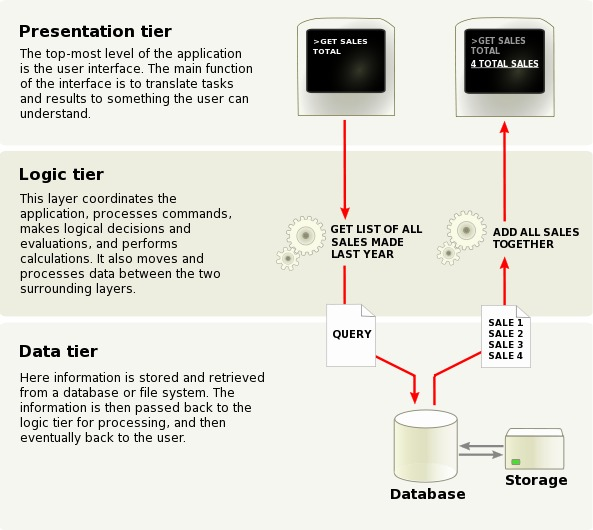
\includegraphics[scale=0.6]{img/3-tier}
    \caption{Architecture trois couches}
	\label{3-tier}
\end{center}
\end{figure}

Dans cette approche, les couches communiquent entre elles au travers d'un « modèle d'échange », et chacune d'entre elles propose un ensemble de services rendus. Les services d'une couche sont mis à disposition de la couche supérieure. On s'interdit par conséquent qu'une couche invoque les services d'une couche plus basse que la couche immédiatement inférieure ou plus haute que la couche immédiatement supérieure (chaque couche ne communique qu'avec ses voisins immédiats).

Le rôle de chacune des couches et leur interface de communication étant bien définis, les fonctionnalités de chacune d'entre elles peuvent évoluer sans induire de changement dans les autres couches. Cependant, une nouvelle fonctionnalité de l'application peut avoir des répercussions dans plusieurs d'entre elles. Il est donc essentiel de définir un modèle d'échange assez souple, pour permettre une maintenance aisée de l'application.

Ce modèle d'architecture 3-tiers a pour objectif de répondre aux préoccupations tels que l'allègement du poste de travail client, la prise en compte de l'hétérogénéité des plates-formes (serveurs, clients, langages, etc.), l'amélioration de la sécurité des données, en supprimant le lien entre le client et les données, la rupture du lien de propriété exclusive entre application et données et enfin, meilleure répartition de la charge entre différents serveurs d'application. \cite{3-tiers}

\subsection{L'architecture Modèle-vue-contrôleur (MVC)}

L'architecture MVC est un motif d'architecture qui sépare la représentation de l'information à partir de l'interaction de l'utilisateur avec elle. Le modèle comprend des données d'application, les règles métier, la logique et les fonctions. Une vue peut être n'importe quelle représentation de sortie de données, comme un graphique ou un diagramme. Plusieurs vues des mêmes données sont possibles, comme un graphique à barres pour la gestion et une vue tabulaire pour les comptables. L'entrée de la médiation du contrôleur, le convertir en commandes pour le modèle ou la vue \cite{mvc}. 

\begin{figure}[h]
\begin{center}
    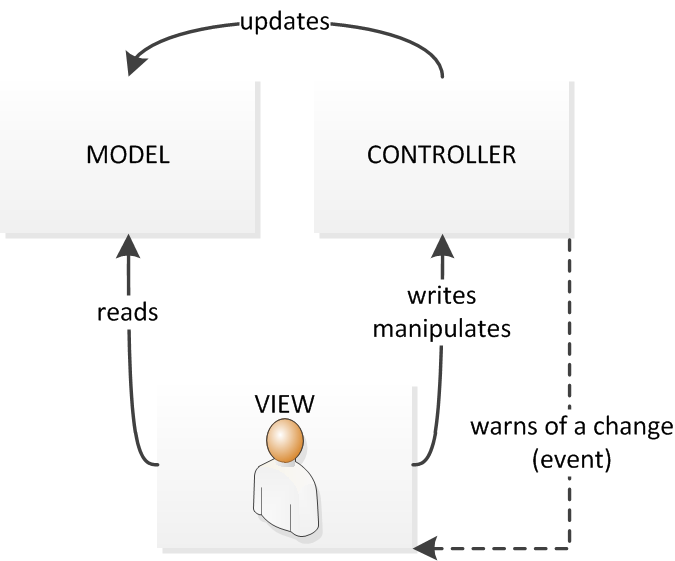
\includegraphics[scale=1.0]{img/mvc}
    \caption{Architecture modèle-vue-contrôleur}
	\label{3-tier}
\end{center}
\end{figure}

Souvent confondue avec l'architecture trois couches, la MVC se distingue dans le fait que l'architecture 3-tiers sépare la couche métier de la couche d'accès aux données. Pour qu'une application MVC soit une vraie application 3-tiers, il faut lui ajouter une couche d'abstraction d'accès aux données de type \textit{DAO} (Data Access Object). Inversement pour qu'une application 3-Tiers respecte MVC il faut lui ajouter une couche de contrôle entre l'interface utilisateur et les règles métier. Loin d'être antagonistes, ces deux pratiques se combinent et sont la fondation de la plupart des frameworks de création d'applications web \cite{mvc-3-tier}.

\subsection{Cas pratique dans le système de gestion CELGMED}

Dans le système de gestion des adhérents à la société d'assurance des employés de la compagnie énergétique de l'état de Goiás, le système trois couches/MVC est représenté par des classes de Vue, Contrôle, Business et Persistance. D'autres classes de support, telles que les  « Vérificateur », étaient aussi présentes, mais plus pour une question d'organisation que de  style d'architecture.

Comme l'on peut voir, ce style est composé à la fois de classes de Présentation/Vue, de Business/Logique/Modèle, de Données/Persistance et de Contrôle, ce qui assure une gestion de donnés et de développement logiciel plus rigoureux que les deux systèmes séparés : si d'un côté il y a plus d'entités qui détiennent un accès limité aux informations, et donc s'il faut écrire plus de lignes de code, de l'autre côté cela assure la modularité du programme et la maintenance du code.

De mode général, ce flux de contrôle se passe de la façon suivante :

\begin{enumerate}
\item L'utilisateur du programme fait une action dans la \textbf{Vue}, ce qui génère un événement
\item Cet événement est capté par Vue et transmis au \textbf{Contrôleur} associé
\item Le Contrôleur fait appel au \textbf{Business}, qui applique la logique du système selon le cas échéant
\begin{itemize}
\item Les \textbf{Vérificateur}s interviennent normalement entre le Contrôleur et le Business, lorsque l'utilisateur fait un action limitée par la conception de la Vue, qui n'a pas de rapport avec la logique intrinsèque du système
\end{itemize}
\item Le Business appelle la \textbf{Persistance} pour consulter ou modifier la base de données du système
\item Une message de confirmation ou d'erreur est transmise dans le flux contraire jusqu'à la Vue et à l'utilisateur.
\end{enumerate}

La table \ref{flux} représente ce flux de manière schématique avec l'exemple d'un utilisateur qui veut consulter tous les clients de la base de données.

\begin{table}[ht]
\begin{center}
    \begin{tabular}{ | p{8.5cm} | p{5cm} |}
    \hline
    \textbf{Flux de contrôle} & \textbf{Classes concernées} \\ \hline
    L'utilisateur clique sur le bouton « Afficher clients »  & \textit{Utilisateur} $\rightarrow$ Vue \\ \hline
    La Vue appelle le Contrôleur afin d'interpréter l'événement clic & Vue $\rightarrow$ Contrôleur \\ \hline
    Le Contrôleur fait usage du Vérificateur pour voir si toutes les champs de saisie de texte ont été bien remplis 
    	(par exemple, n'a-t-il pas mis de caractères de l'alphabet dans le champ « période de consultation » ?)
    	En cas positif, il appelle le Business ; sinon, un message d'erreur se produit et l'utilisateur réécrit les informations. 
    	& Contrôleur $\rightarrow$ (Vérificateur) $\rightarrow$ Business \\ \hline
    Le Business vérifie la logique du système (par example, est-ce que l'utilisateur a le droit d'accès à 
    \textit{tous} les clients de la base de données ?).
    	Ensuite, il appelle la Persistance pour retrouver l'information correspondante
    	& Business  $\rightarrow$ Persistance \\ \hline
    La persistance utilise des commandes SQL pour consulter la base de données et retrouver les clients indiqués par le Business 
    	(par example, les clients supprimés ne seront pas affichés). 
    	La réponse de cette requête est donc renvoyé dans le flux inversé jusqu'à la Vue. 
    	& Persistance $\rightarrow \cdots \rightarrow$ Vue \\ \hline
    La Vue organise l'information et la rend visible à l'utilisateur, sous forme de table mise en forme 
    	& Vue $\rightarrow$ \textit{Utilisateur} \\
    \hline
    \end{tabular}
\end{center}
\caption{Flux de contrôle dans l'architecture des systèmes Asert}\label{flux}
\end{table}